\chapter[Perspectiva]{Perspectiva}

\section{Incremento atual}
  \subsection{Estrutura}
    \begin{enumerate}
      \item Modelagem da cadeira motorizada adaptada: Foi feito a modelagem da cadeira de rodas levando em conta a solução de portabilidade e acessibilidade da mesma, pontuando pontos como o design de inovação do anexo autômato a cadeira;
      \item Escolha do material a ser usado em anexo: Um estudo dos possíveis materiais será realizado, alavancando os motivos e vantagens do uso dos mesmos para suporte das cargas;

      \item Ergonomia do produto: Estudo e modelagem do melhor design da cadeira de rodas manual com o anexo que a motoriza;

      \item Desenvolvimento de um modelo de PVC para testes do sistema de acoplamento;

      \item Desenvolvimento do eixo que ira transmitir potência entre a roda ao conjunto de moto-redução.

    \end{enumerate}
  \subsection{Power Train}
    \begin{enumerate}
      \item Escolha do motor elétrico quanto ao custo do mesmo no projeto, embasado em estudo feito em relação a peso, velocidade máxima, velocidade nominal;
      \item Especificação do motor elétrico de Corrente Contínua quanto a potência minima;
      \item Estudo e especificação sobre baterias a serem utilizadas, quanto tensão, capacidade e dimensão. Foi escolhido usar as baterias de Chumbo-Ácida selada, levanto em conta vantagens e limitações. Os cálculos de autonomia foram feitos para melhor estimar o método de carregamento da bateria;

 	\item Estudo com o auxílio do software Matlab da interferência da roda e do peso do sistema no desempenho do conjunto de moto-redução;
 	\item Foram adquirido dois conjuntos de moto-redução  pela empresa MKS Redutores de São Paulo. O motor com redutor escolhido para o projeto foi o MR com motor GPB que possui as seguintes especificações com potência de 305 a 350 W e redução de 1:10.

    \end{enumerate}

    \subsection{Controle}
      \begin{enumerate}
        \item Especificação de tecnologia: Estudo e escolha da melhor tecnologia voltada para o problema, que no caso será feito com um Raspberry Pi para comunicação entre a interface do usuário e o motor;

        \item Controle de potência: Estudo de qual tipo de controlador de potência a ser usado no motor, para controle de sua corrente. A escolha da utilização da ponte H será combinado com o algoritmo de PWM, que utiliza o Raspberry Pi como forma de resposta aos comandos dos usuários como a diração, aceleração, frenagem da cadeira motorizada adaptada;

        \item Escolha da linguagem de programação: Definição de qual linguagem será utilizada com base na problemática existente e nos recursos a serem utilizados. A linguagem escolhida foi o Phyton, pois existem bibliotecas especificas que controlam GPIO do Raspebery Pi.

      \end{enumerate}

  \subsection{Interface com Usuário}
    \begin{enumerate}
      \item Estudo de tecnologias para interfaces: Estudo de quais tecnologias são usadas como interface de usuário para controle da cadeira motorizada adaptada. Neste estudo são observados dispositivos de controle como Joystick e aplicativos que podem utilizar tecnologia Bluetooth ou VPN para comunicar com o Raspberry Pi.

      \item Escolha da linguagem de programação do aplicativo: Definição de qual linguagem será utilizada com base na problemática existente e nos recursos a serem utilizados. A linguagem escolhida para o desenvolvimento do aplicativo será definida conforme o resultado de estudo de utilziação de Bluetooth e VPN. Caso a escolha seja para dispositivos Android, então pode ser escolhida a linguagem nativa Java, caso a escolha seja para dispositivos iOS, então pode ser escolhida a linguagem nativa Objective-C ou Swift.

    \end{enumerate}

\section{Próximos passos}
  \subsection{Estrutura}
    \begin{enumerate}
      \item Testes com o eixo acoplado ao motor;
      \item Escolha de material mediante norma ABNT 6061 - T6;
	 \item Desenvolvimento do protótipo.
    \end{enumerate}
  \subsection{Power Train}
    \begin{enumerate}
      \item Testes em conjunto com a parte de estrutura e controle.
      \end{enumerate}

  \subsection{Interface com Usuário}
    \begin{enumerate}
      \item Montagem do Joystick ergonômico.
    \end{enumerate}
  \subsection{Controle}
    \begin{enumerate}
     \item Implementação de filtro para suavizar movimentos do Joystick para motores;
     \item Implementação dos testes para os códigos do MSP;
     \item Implementação dos sensores de nível de bateria e velocidade em MSP;
    \end{enumerate}

\section{Cronograma}

  Para prosseguir com os próximos passos um cronograma com as estimativas de cada Sprint foi levantado.

  \begin{figure}[!htb]
  \centering
    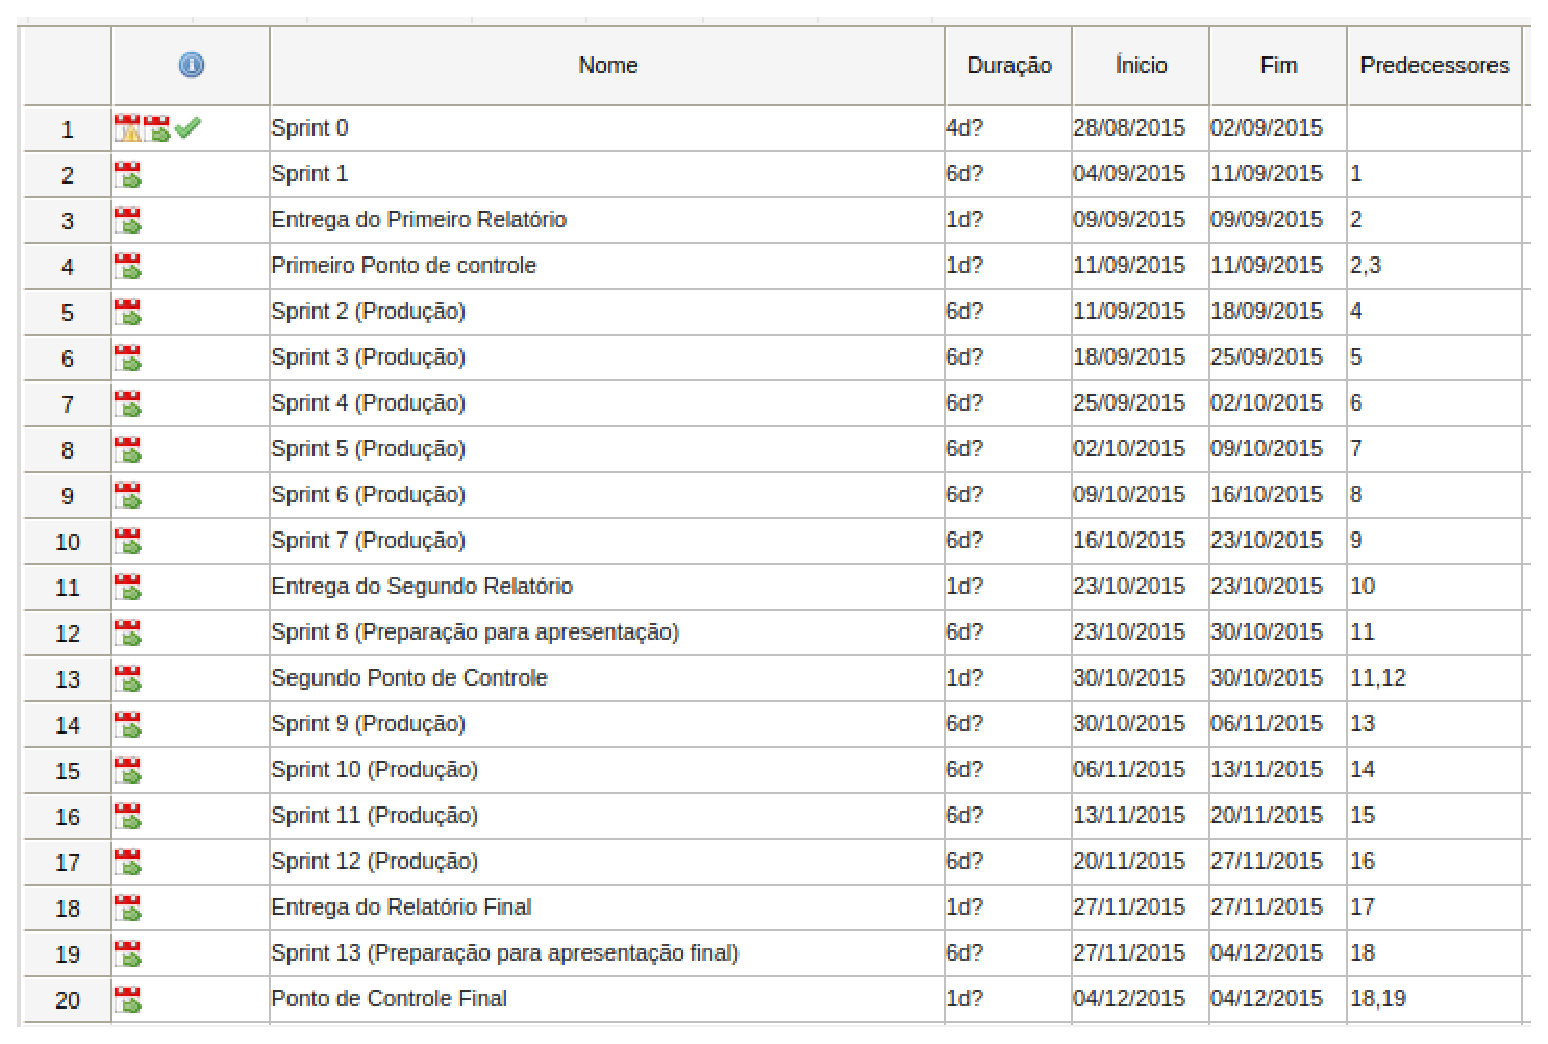
\includegraphics[keepaspectratio=true,scale=0.5]{figuras/metodologia/cronograma}
  \caption{Cronograma}
  \label{fig:cronograma}
  \end{figure}
